% main.tex

\documentclass[conference,10pt]{IEEEtran}

\usepackage[T1]{fontenc}
\usepackage[utf8]{inputenc}
\usepackage[spanish,es-noindentfirst]{babel}
\usepackage{multirow}
\usepackage{microtype}
\usepackage{graphicx}
\usepackage{booktabs}
\usepackage{siunitx}
\usepackage{subcaption}
\usepackage{xcolor}
\usepackage{amsmath}
\usepackage{placeins}
\usepackage{float}
\usepackage{threeparttable}
\usepackage[hidelinks]{hyperref}
\usepackage[capitalise,noabbrev]{cleveref}

\addto\captionsspanish{\renewcommand{\tablename}{Tabla}}
\addto\captionsspanish{\renewcommand{\IEEEkeywordsname}{Palabras clave}}
\crefname{figure}{figura}{figuras}\Crefname{figure}{Figura}{Figuras}
\crefname{table}{tabla}{tablas}\Crefname{table}{Tabla}{Tablas}
\crefname{section}{sección}{secciones}\Crefname{section}{Sección}{Secciones}
\crefname{equation}{ec.}{ecs.}\Crefname{equation}{Ec.}{Ecs.}
\AtBeginDocument{%
  \renewcommand{\crefpairconjunction}{ y }%
  \renewcommand{\creflastconjunction}{ y }%
  \renewcommand{\crefrangeconjunction}{ a }}

\sisetup{round-mode=places,round-precision=2,detect-weight=true}
\graphicspath{{figures/}{images/}}

\begin{document}

\title{Impacto de las Épocas Offline en el Rendimiento y la Exactitud de Entrenamientos Distribuidos con O.N.O.}

\author{\IEEEauthorblockN{Marcos Bianchi}
\IEEEauthorblockA{Facultad de Ingeniería, Universidad de Buenos Aires\\
Aprendizaje Profundo\\
Julio 2026}}

\maketitle

% abstract.tex

\begin{abstract}
Retrasar la sincronización entre nodos en un entrenamiento distribuido reduce la frecuencia de comunicación pero induce divergencia entre los pesos (\emph{client drift}). Este trabajo evalúa el impacto de variar las épocas offline ($E$) utilizando el sistema de entrenamiento O.N.O. bajo las topologías \emph{Parameter Server} sincrónico y \emph{All-Reduce (ring)}. Los experimentos se ejecutaron sobre un clúster de contenedores Docker con emulación de red mediante Pumba. Entrenando LeNet-5 sobre MNIST FULL, los resultados muestran que incrementar $E$ no aporta reducciones significativas en los tiempos totales debido a la contención del hardware local, mientras que degrada la \emph{accuracy} final e incrementa la inestabilidad de la pérdida durante el entrenamiento.
\end{abstract}

\begin{IEEEkeywords}
Épocas Offline, Parameter Server, All-Reduce, O.N.O., Client Drift, Pumba.
\end{IEEEkeywords}

\section{Introducción y Objetivos}

En entrenamientos paralelizados por datos, la sincronización frecuente entre los distintos nodos degrada la velocidad del entrenamiento. Permitir que los nodos operen de forma más autónoma durante algunas épocas posterga el intercambio de gradientes y parámetros, disminuyendo así su dependencia en la red durante el entrenamiento y focalizando el tiempo de cómputo en el cálculo de gradientes y optimización del modelo.

\textbf{Pregunta de investigación.} ¿Cómo impactan las épocas offline a la velocidad y eficacia del modelo entrenado?

\textbf{Objetivos.} Evaluar esta pregunta utilizando O.N.O., un sistema de entrenamiento distribuido de modelos de aprendizaje profundo que implementamos junto a mis compañeros para nuestro trabajo práctico profesional como trabajo de fin de carrera. Con ello ejecutar varios entrenamientos sobre una misma arquitectura, dataset e hiperparámetros para relevar las diferencias en cuanto al impacto real de las épocas offline.

% architecture.tex

\section{Arquitectura del Sistema y Mecanismos de Sincronización}

\subsection{Componentes Principales de O.N.O.}
\begin{itemize}
    \item \textbf{Orchestrator:} Mediante una configuración declarativa del entrenamiento brindada por el usuario, configura al resto de nodos para iniciar el entrenamiento de un modelo usando alguno de los algoritmos implementados. Al finalizar un entrenamiento, consolida los resultados parciales generando un archivo \emph{safetensors} que contiene los parámetros del modelo entrenado. Para una mejor automatización, cuenta con una interfaz FFI de Python que fue utilizada para orquestar los ensayos discutidos más adelante.
    \item \textbf{Workers:} Computan gradientes locales por \emph{backpropagation} sobre una partición asignada del dataset. En \emph{All-Reduce} aplican localmente el optimizador, mientras que en \emph{Parameter Server} delegan la actualización a los servidores.
    \item \textbf{Servers:} Nodos dedicados al almacenamiento y optimización de parámetros del modelo. Reciben gradientes parciales de los \emph{workers}, los agregan y aplican sobre los parámetros para luego redistribuirlos.
\end{itemize}

\subsection{Dinámica de Sincronización Demorada ($E > 1$)}
Al parametrizar $E > 1$, los nodos ejecutan $E$ épocas de entrenamiento de forma autónoma antes de realizar un intercambio de red. El tráfico de comunicación se reduce considerablemente de forma inversamente proporcional a $E$. No obstante, la falta de sincronización continua causa que los pesos locales de los \emph{workers} diverjan (\emph{client drift}). Al alcanzar la fase de sincronización, la consolidación se realiza agregando los gradientes acumulados durante dicho período.

Bajo un entrenamiento optimizado por \emph{Gradient Descent}, la actualización del vector de parámetros global tras un intervalo de sincronización se modela como:

\begin{equation}
W_{t + E} = W_{t} - \frac{\lambda}{N} \sum_{i=1}^{N} G_{i}^{(E)}
\end{equation}

donde $N$ es el número de \emph{workers}, $\lambda$ es el \emph{learning rate} y $G_{i}^{(E)}$ representa la acumulación de gradientes calculados por el \emph{worker} $i$ a lo largo de las $E$ épocas locales.

\subsection{Algoritmos de Entrenamiento Distribuido}
El sistema implementa distintos algoritmos de comunicación distribuida, centrándose este trabajo en:

\begin{itemize}
    \item \textbf{Parameter Server Sincrónico:} Algoritmo centralizado basado en el modelo propuesto por Li et al.~\cite{li2013parameter}. Una barrera de sincronización bloquea a los \emph{workers} hasta que los \emph{servers} procesan el lote global de gradientes, garantizando que todos los nodos inicien el siguiente ciclo desde el mismo estado de parámetros.
    \item \textbf{All-Reduce (Ring):} Algoritmo descentralizado inspirado en arquitecturas de alto rendimiento como Horovod~\cite{sergeev2018horovod}. Los \emph{workers} se organizan en una topología de anillo lógico y comparten fragmentos de gradientes en fases sucesivas de \emph{scatter} y \emph{gather}, actualizando de forma idéntica y local el vector de parámetros resultante.
\end{itemize}

\begin{figure*}[!t]
    \centering
    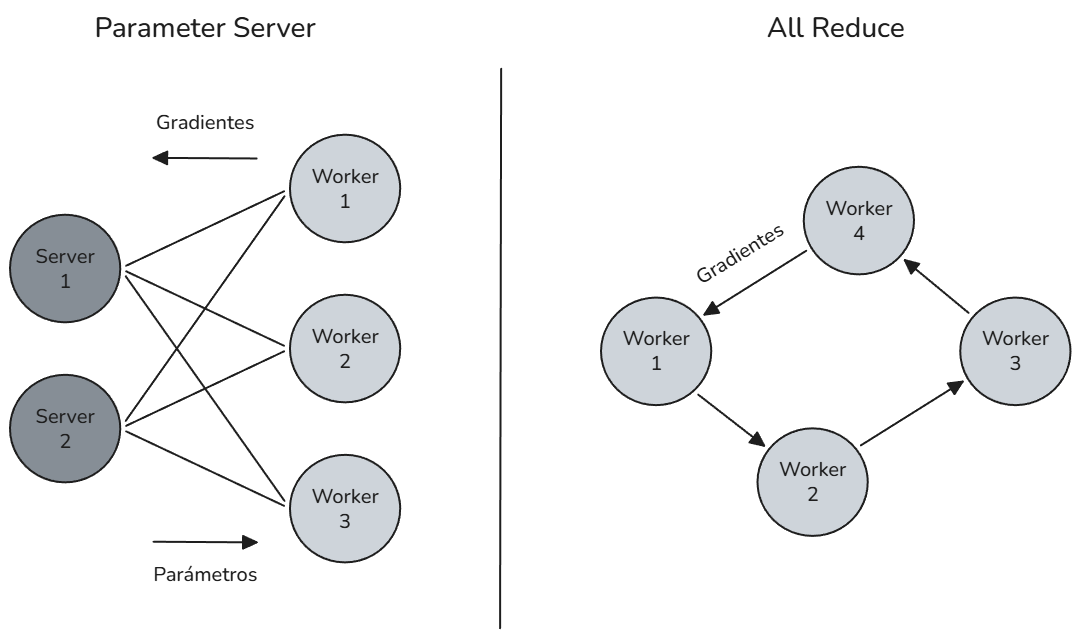
\includegraphics[width=0.75\textwidth]{topologies} 
    \caption{Topologías distribuidas soportadas en O.N.O. (Izquierda) Arquitectura centralizada bajo \emph{Parameter Server} donde los \emph{workers} obtienen parámetros y envían gradientes a \emph{servers} fragmentados. (Derecha) Topología descentralizada en anillo \emph{All-Reduce} donde los nodos se comunican de forma punto a punto con sus vecinos adyacentes.}
    \label{fig:topologias_ono}
\end{figure*}


\section{Metodología Experimental}
Todos los entrenamientos fueron realizados en la misma computadora de forma secuencial utilizando Docker para simular un entorno multicomputadora, sumando un total de \num{10.5} horas de ejecución. Las especificaciones técnicas del entorno se detallan en la \Cref{tab:environment}, mientras que las variables lógicas y configuraciones del modelo O.N.O. se consolidan en la \Cref{tab:configs}.

\begin{table}[ht]
	\caption{Configuración de Ensayos}
	\label{tab:configs}
	\centering
	\footnotesize
	\begin{tabular}{llp{2.4cm}}
		\toprule
		\textbf{Categoría} & \textbf{Parámetro} & \textbf{Valores Evaluados} \\
		\midrule
		\multirow{3}{*}{Modelo y Datos} & Dataset & MNIST (Full)~\cite{lecun1998gradient} \\
		 & Arquitectura de Red & LeNet-5 \\
		 & Función de Pérdida & Entropía Cruzada \\
		\midrule
		\multirow{3}{*}{Optimización} & Optimizador & Adam \newline $\alpha = 0.01 \newline \beta_1 = 0.9 \newline \beta_2 = 0.999 \newline \epsilon = 10^{-8}$ \\
		 & Tamaño de Mini-Batch & 64 \\
		 & Épocas Máximas & 48 \\
		\midrule
		Infraestructura & Serialización & Sparse ($r = 0.5$) \\
		\midrule
		\multirow{3}{*}{Variables Libres} & Algoritmo Distribuido & All-Reduce, Parameter Server (Sincrónico/Bloqueante) \\
		 & Nodos & 2, 4, 6, 8, 10 \\
		 & Épocas Offline & 0, 1, 2, 3, 4 \\
		\bottomrule
	\end{tabular}
	\begin{tablenotes}
		\item[*] Para el algoritmo de \emph{Parameter Server}, el total de nodos se compone de forma que la mitad de ellos son \emph{workers} y la otra \emph{servers}.
	\end{tablenotes}
\end{table}

\subsection{Compresión de Red: Serialización Sparse}
La configuración de la sección de infraestructura responde al método de serialización de gradientes del sistema, el cual soporta una variante \emph{sparse} (o dispersa) diseñada para optimizar la comunicación distribuida limitando el intercambio de sectores poco impactantes de los gradientes~\cite{aji-heafield-2017-sparse}. El parámetro $r$ sirve para acotar el sampleo del gradiente que se quiere transmitir: a mayor $r$, mayor será la compresión teórica. 

El algoritmo calcula la cardinalidad efectiva del mensaje mediante:

\begin{equation}
k = \text{round}\left(|g| \cdot (1.0 - r)\right)
\end{equation}

El valor resultante $k$ se utiliza para escoger los $k$ elementos de mayor magnitud absoluta dentro del tensor de gradientes local, fijando un umbral mínimo. Todo valor que alcance o supere dicho umbral se incorporará al mensaje por enviar. De esta forma, un valor de $r = 0.0$ samplea la totalidad del gradiente, mientras que un $r = 0.5$ (como el configurado para estos experimentos) filtra el \SI{50}{\percent} de los componentes para disminuir el transito por red. Los elementos descartados se acumulan en un gradiente residual para ser considerados en el próximo mensaje.

\begin{table}[ht]
	\caption{Entorno de Ejecución}
	\label{tab:environment}
	\centering
	\footnotesize
	\begin{tabular}{llp{2.4cm}}
		\toprule
		\textbf{Categoría} & \textbf{Componente} & \textbf{Detalle} \\
		\midrule
		\multirow{5}{*}{Procesador} & Modelo & Intel Core i5-8350U \\
			& Arquitectura & x86\_64 \\
			& Núcleos Físicos & 4 \\
			& Hilos Lógicos & 8 \\
			& Frecuencia de Reloj & Base: \SI{1.7}{\giga\hertz} \newline Turbo: \SI{3.6}{\giga\hertz} \\
		\midrule
		\multirow{2}{*}{Memoria} & Capacidad Total RAM & 8 GB \\
			& Tipo & DDR4 \\
			& Velocidad & \SI{2400}{\mega\hertz} \\
		\midrule
		\multirow{2}{*}{Entorno de Software} & Sistema Operativo & Ubuntu 24.04 LTS \\
			& Entorno de Ejecución & Docker v29.6.1 \newline Rust v1.96.1 \newline CPython v3.14.0 \\
		\bottomrule
	\end{tabular}
\end{table}

\FloatBarrier


\section{Resultados y Análisis Experimental}

\subsection{Análisis Temporal y Escalabilidad del Hardware}

La variación de $E$ no trajo ningún tipo de mejora apreciable en el tiempo de ejecución de los entrenamientos, las curvas de cada configuración se solapan en todas las pruebas. Dado que el sistema se ejecuta sobre una sola máquina tiene sentido que no haya una gran diferencia en tiempo, aunque sí me esperaba algún tipo de mejora.

\begin{figure}[H]
  \centering
  
\includegraphics[width=0.5\textwidth]{all_reduce/execution_time_summary}
  \caption{Comparación de tiempos de ejecución bajo distintas cantidades de Épocas Offline con All Reduce.}
  \label{fig:all_reduce_tiempos}
\end{figure}

Como se observa en la \Cref{fig:all_reduce_tiempos}, el rendimiento escalable se estanca al superar los 4 nodos. En All Reduce, escalar a 10 nodos llegó a degradar la performance debido al alto nivel de contención sobre el CPU.

\begin{figure}[H]
  \centering
  
\includegraphics[width=0.5\textwidth]{parameter_server/execution_time_summary}
  \caption{Comparación de tiempos de ejecución bajo distintas cantidades de Épocas Offline con Parameter Server.}
  \label{fig:parameter_server_tiempos}
\end{figure}

Se aprecia facilmente en la \Cref{fig:parameter_server_tiempos} que el sistema aún con 10 nodos (5 \emph{workers} y 5 \emph{servers}) consigue mejorar su tiempo previo con menor cantidad de nodos. A diferencia de \emph{All Reduce}, donde los nodos están constantemente procesando datos, \emph{Parameter Server} tiene momentos de tiempo muerto, por ejemplo, en la variación sincrónica utilizada, donde en el momento en el que el \emph{server} está optimizando el modelo sabemos que el resto de workers tienen que estar bloqueados en la barrera interna del servidor. Esto le cede hilos de ejecución a los nodos \emph{server}, por lo que se aprovecha mejor tener más de un tipo de entidad por computadora, o en este caso, CPU.

Es importante notar que ya de entrada All Reduce es más rápido que Parameter Server, esto tiene sentido porque All Reduce aprovecha mejor la distribución de responsabilidades y cada nodo está constantemente procesando datos, ya sea calculando gradientes, compartiendolos u optimizando los parámetros.

\subsection{Métricas de Exactitud}

En cuanto a resultados de accuracy, la variación de $E$ se puede apreciar mucho mejor ya que no depende del hardware en donde se esté ejecutando el entrenamiento. Se aprecian mucho mejor estos resultados que los anteriores.

Consistentemente para ambos algoritmos el modelo resultante es peor en cuanto a accuracy a medida que $E$ incrementa, lo cual no me sorprende para nada, en cuanto a que tán peor es, teniendo en cuenta que introducir tan solo 1 época offline ya reduce la cantidad de sincronizaciones en la red a la mitad, este deterioro es tan solo del ~1\%.

Si los entrenamientos fueran ejecutados en un entorno real, creo yo que se podría entender mejor que tan superior es incrementar $E$, por ejemplo, llegar a ejecutar más épocas totales en la misma cantidad de tiempo, ¿Podría un setup como ese superar a uno que sincronize en todas las épocas?

\begin{figure}[H]
  \centering
  
\includegraphics[width=0.5\textwidth]{parameter_server/accuracy_summary}
  \caption{Comparación de accuracy bajo distintas cantidades de Épocas Offline con Parameter Server.}
  \label{fig:parameter_server_accuracy}
\end{figure}

Como mencioné antes, se nota un degradamiento en la accuracy a mayor $E$. Lo que si puede ser interesante es que a medida que incrementa la cantidad de nodos, esto se hace más notable, lo cual tiene sentido si pensamos que a medida que la cantidad de nodos aumenta, también aumentan las particiones de datasets y esto las hace cada vez mas chicas. El \emph{Orchestrator} termina repartiendo particiones de dataset cada vez más chicas y potencialmente más sesgadas, por lo que tener menos sincronización de parámetros en los \emph{workers} termina perjudicando aún más al fin del día.

\begin{figure}[H]
  \centering
  
\includegraphics[width=0.5\textwidth]{all_reduce/accuracy_summary}
  \caption{Comparación de accuracy bajo distintas cantidades de Épocas Offline con All Reduce.}
  \label{fig:all_reduce_accuracy}
\end{figure}

Hablando de \emph{All Reduce}, la degradación de la accuracy en relación a la cantidad de nodos y $E$ es todavía más notable que en \emph{Parameter Server}. En cada uno de los setups empleados, \emph{All Reduce} siempre tuvo el doble de \emph{workers} (ya que no tiene \emph{servers}). Esto implica dividir más los datasets y aún más independencia de cada uno de ellos con respecto al resto.

Sincronizar los parámetros y/o gradietes de forma tan tardía también provoca que sus promediados introduzcan correcciones más fuertes y abruptas, generando una desestabilización en el descenso por el gradiente de la función de pérdida y resultando en un peor modelo resultante.

\subsection{Inestabilidad de Pérdida durante el Entrenamiento}

Mediante las historias de pérdida de los entrenamientos realizados, junté un par que me parecieron buenos para relevar algunos puntos importantes. Como mencioné anteriormente, esperaba que incrementar $E$ introdujera inestabilidad en el entrenamiento.

Para los entrenamientos realizados en \emph{All Reduce} y \emph{Parameter Server} de 2 nodos se nota esta inestabilidad en forma de picos cada vez más pronunciados a medida que crece $E$.

\begin{figure}[H]
  \centering
  
\includegraphics[width=0.5\textwidth]{parameter_server-2/loss_history_per_offline_epoch}
  \caption{Trayectoria de Loss en Entropía Cruzada exchibiendo ruido estocástico por cómputo offline en Parameter Server (2 nodos).}
  \label{fig:parameter_server_loss}
\end{figure}

Es claro que al optimizador le cuesta más al comienzo, ya que suele ser la etapa de corrección más grande del entrenamiento, una vez que encuentra un mínimo local se estabiliza y converge. Notar que cada vez converge a valores más altos, ¿Será que a mayor $E$ no es posible o dificulta al optimizador de alguna forma a no alcanzar nunca el mínimo local verdadero? Al estilo de tener un alto valor de \emph{learning rate} en el que el optimizador podría quedar oscilando sobre el mínimo sin nunca alcanzarlo.

\begin{figure}[H]
  \centering
  
\includegraphics[width=0.5\textwidth]{all_reduce-2/loss_history_per_offline_epoch}
  \caption{Trayectoria de Loss en Entropía Cruzada exchibiendo ruido estocástico por cómputo offline en All Reduce (2 nodos).}
  \label{fig:all_reduce_loss}
\end{figure}

Para \emph{All Reduce} sucede algo parecido aunque parece más controlado, sinceramente esperaba lo contrario, hayar mayor inestabilidad con este algoritmo que con \emph{Parameter Server}, se ve que se mantuvo más estable.

\section{Discusi\'on y Limitaciones}
Las ventajas del c\'omputo offline est\'an estrictamente atadas a la latencia real de la red f\'isica. En un entorno local compartido mediante Docker, eliminar el overhead de mensajes no compensa el costo matem\'atico del desv\'io de gradientes, pagando una penalizaci\'on severa de precisi\'on sin retornos temporales. 

En contraposici\'on, en cl\'usters distribuidos reales (multi-m\'aquina sobre LAN/WAN), retrasar la agregaci\'on resulta cr\'itico para amortizar la latencia f\'isica de sockets e interrupciones de E/S. El compromiso final debe ajustarse evaluando el tama\~no del modelo y la velocidad de interconexi\'on.

\section{Conclusi\'on}
El uso de \'epocas offline en O.N.O. modula el balance b\'asico entre demandas de comunicaci\'on y fidelidad algor\'itmica del modelo. En la infraestructura local simulada, incrementar $E$ inestabiliz\'o el entrenamiento de LeNet-5 de manera predecible sin aportar ganancias de velocidad, debido a las limitantes de hardware de la CPU hospedadora de 4 cores f\'isicos. 

El estudio evidencia el valor del sistema para diagnosticar fallas de escalabilidad l\'ogica y comportamientos asint\'oticos de optimizadores. Como trabajo futuro, se plantea validar el sistema bajo topolog\'ias multi-nodo reales con latencias de red inducidas por software.


\nocite{*} 
\bibliographystyle{IEEEtran}
\bibliography{references}

\end{document}
